\begin{frame}{Context}{Multi-agent Simulation of Smart Cities}
Application of multi-agent \alert{simulations} in the field of smart cities and smart islands. Example of London and Reunion Island cases. Collaboration with 
    \begin{figure}
	
\includegraphics[width=2cm]{assets/icl.png}
	\hspace{2cm}
	
\includegraphics[width=1cm]{assets/saintDenis.png}
    \end{figure}

\note{
Cette thèse s'inscrit dans le cadre d'un sous-thème développé par notre groupe de travail système collectif adaptatif (SCA) sur lequel nous travaillons avec des chercheurs de l'Imperial College London et la mairie de Saint-Denis de La Réunion. Dans ce cadre nous avons développé deux modèles de simulations multi-agents que nous avons particulièrement appliqué sur Londres et sur La Réunion. Nous travaillons sur 2 modèles de simulations multi-agents.
}
    
\end{frame}

\begin{frame}{Context}{Simulation Models}
\begin{figure}
    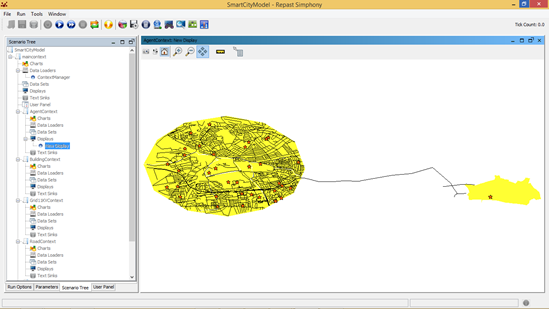
\includegraphics[width=.6\linewidth]{figures/smartCityModel.png}
    \caption{\textbf{SmartCityModel}\footnote{
    RALITERA, Tahina, FERARD, Maxime, BUSTOS-TURU, Gonzalo, et al. Steps Towards Simulating Smart Cities and Smart Islands with a Shared Generic Framework. In : Proceedings of the 6th International Conference on Smart Cities and Green ICT Systems. SCITEPRESS-Science and Technology Publications, Lda, 2017. p. 329-336.
    \medbreak
    RALITERA, Tahina et COURDIER, Rémy. Toward Smart Island Simulation Application. In : International Conference on Practical Applications of Agents and Multi-Agent Systems. Springer, Cham, 2017. p. 457-469.
    } built upon the \textbf{Repast Simphony} multi-agent simulation platform} 
\end{figure}
\note{


\par Le premier esr SmartCityModel : qui a été utilisé pour différents scénario mais qui dans notre cadre a été utilisé pour la simulation de flux de mobilité de véhicules électriques sur un territoire. Il s'agit d'un modèle développé à l'origine par les chercheurs de l'ICL sur lequel nous avons contribué. Cela a notamment fait l'objet de deux publications. Ce modèle de simulation tourne sur la plateforme développée à l'internationale Repast Simphony. Vous pouvez notamment voir ici une capture d'écran de l'interface utilisateur de la simulation. Les agents sont des conducteurs de véhicules électriques ou/et des bornes de recharges électriques. Les voitures électriques sont affichées sous forme d'étoiles orange, ils se déplacent le long des routes qui sont affichées sous forme de lignes noirs.
}
\end{frame}

\begin{frame}{Context}{Simulation Models}

\begin{figure}
    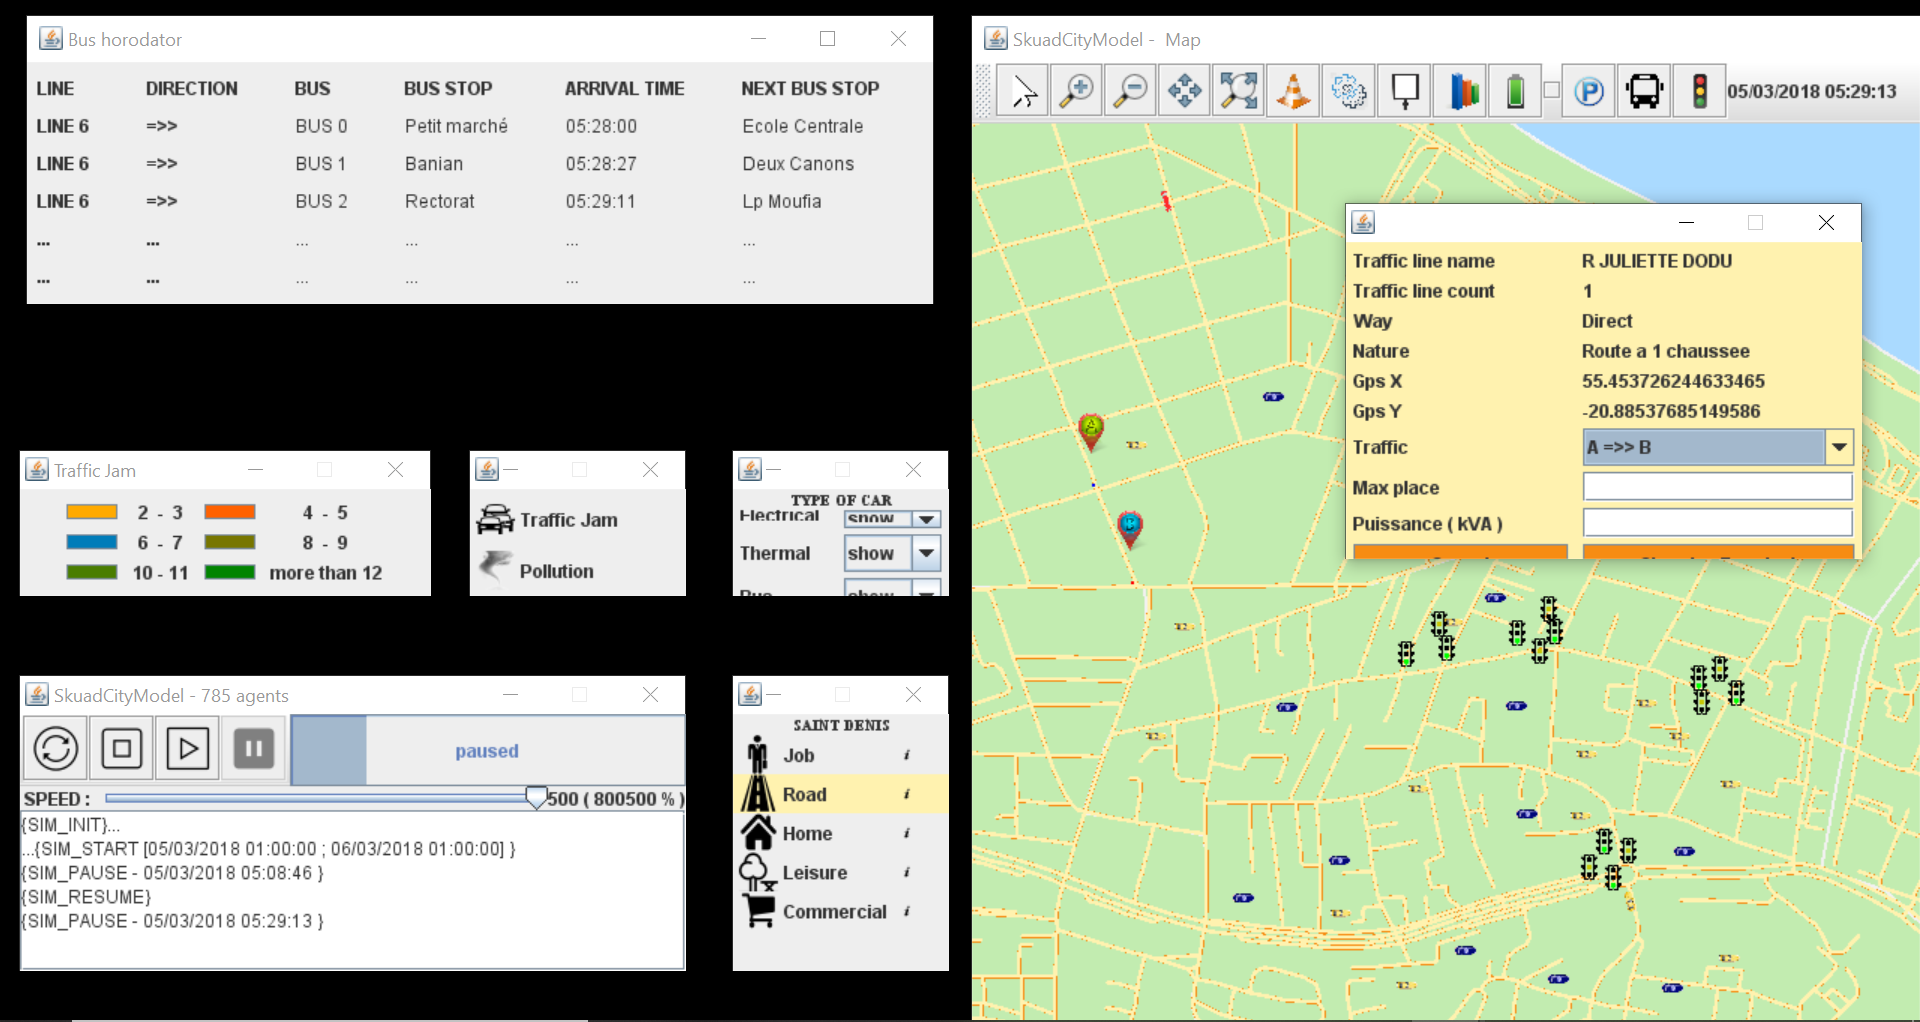
\includegraphics[width=.6\linewidth]{figures/skuadCityModelGUI.png}
    \caption{\textbf{SkuadCityModel}\footnote{AKY, Nathan, TAHINA, Ralitera, PAYET, Denis, et al. SkuadCityModel: Une simulation de déplacements urbains construite sur la plate-forme SKUAD. In : Journées Francophones Systèmes Multi-Agents (JFSMA'16)-Demonstration. Cepadues, 2018. p. 233-234.} built upon the \textbf{SimSKUAD} multi-agent simulation platform}
\end{figure}

\note{
\par  SkuadCityModel : est un modèle développée par notre équipe de travail. Il est inspirée de SmartCityModel et tourne sur SimSKUAD, une plateforme de simulation développée au sein de notre équipe. Voici une capture d'écran de l'interface utilisateur de la simulation. Vous pouvez notamment voir les voitures thermiques en bleu, électriques en jaune, les bornes de recharges électriques, les bâtiment, les routes ainsi que les feu de signalisation.
\par Tout cet environnement spatial que vous pouvez voir sur les captures d'écran est modélisé sur la base de données réelles sous format SIG.

}
\end{frame}

\begin{frame}{Context}{A wealth of untapped information on temporal behaviours}
\begin{figure}
    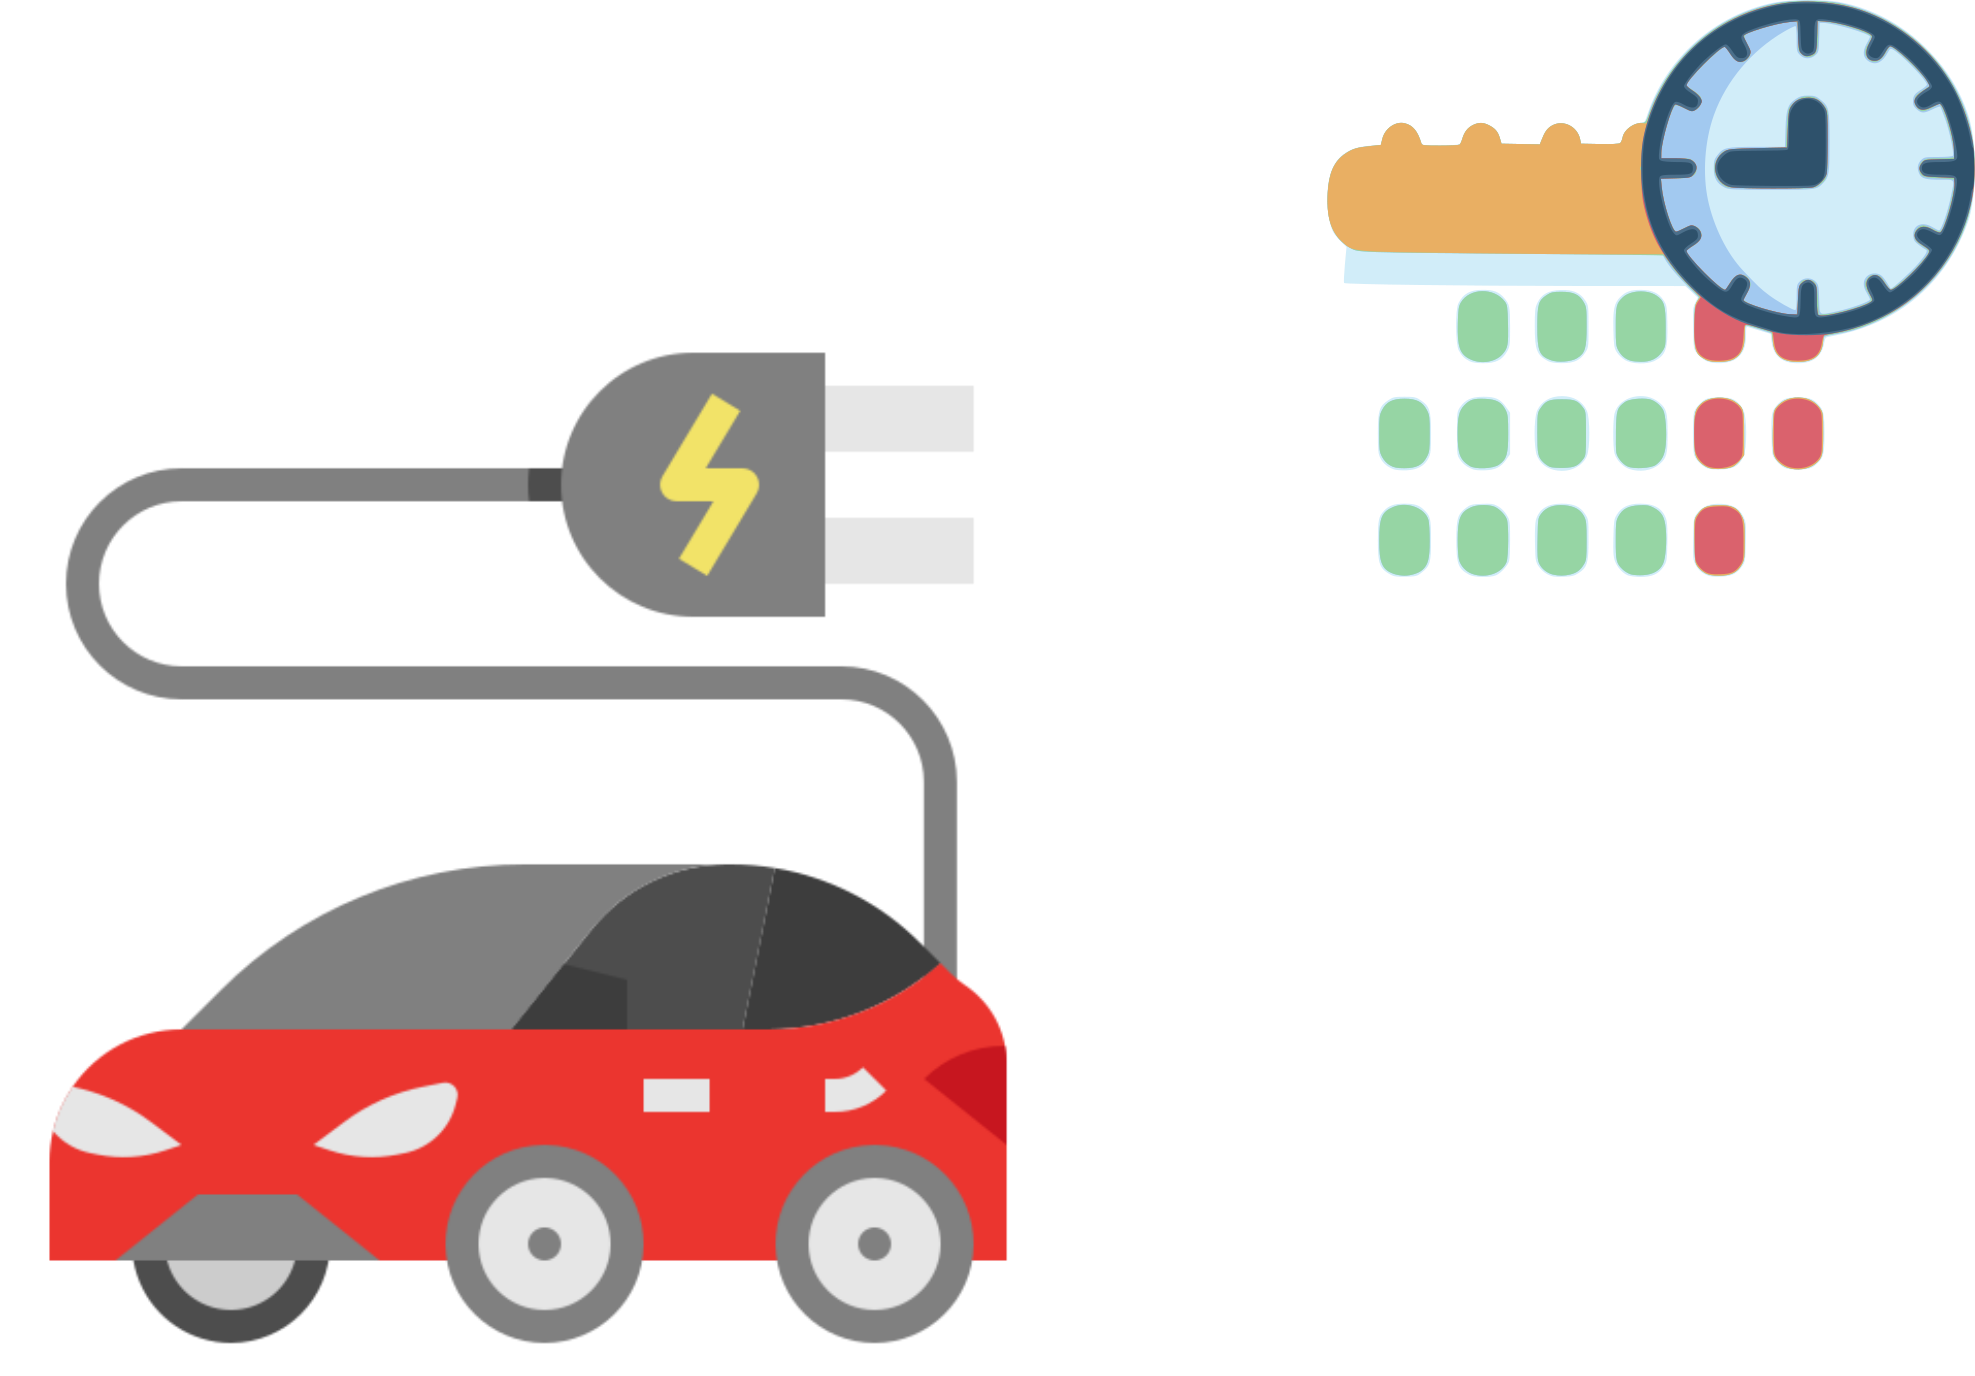
\includegraphics[width=.5\linewidth]{figures/planning.png}
\end{figure}
\par Activity-based model
        \begin{itemize}
            \item the movements result from the activities that the agents wish or have to perform
            \item the agents own an activity planning
        \end{itemize}
\note{
\par Par ailleurs, ces modèles sont des modèles basées sur les activités, c'est-à-dire que les déplacements des véhicules électriques résultent des activités que les agents souhaitent ou doivent effectuer. Les agents disposent alors d'un planning d'activités plus ou moins défini à l'avance. Ce planning est également défini à partir de données statistiques réelles.
\par Nous pouvons donc constater une richesse d'information que nos agents peuvent exploiter au niveau de leur raisonnements. 

}
\end{frame}

\begin{frame}{Context}{A wealth of untapped information on temporal behaviours}
    \begin{figure}
    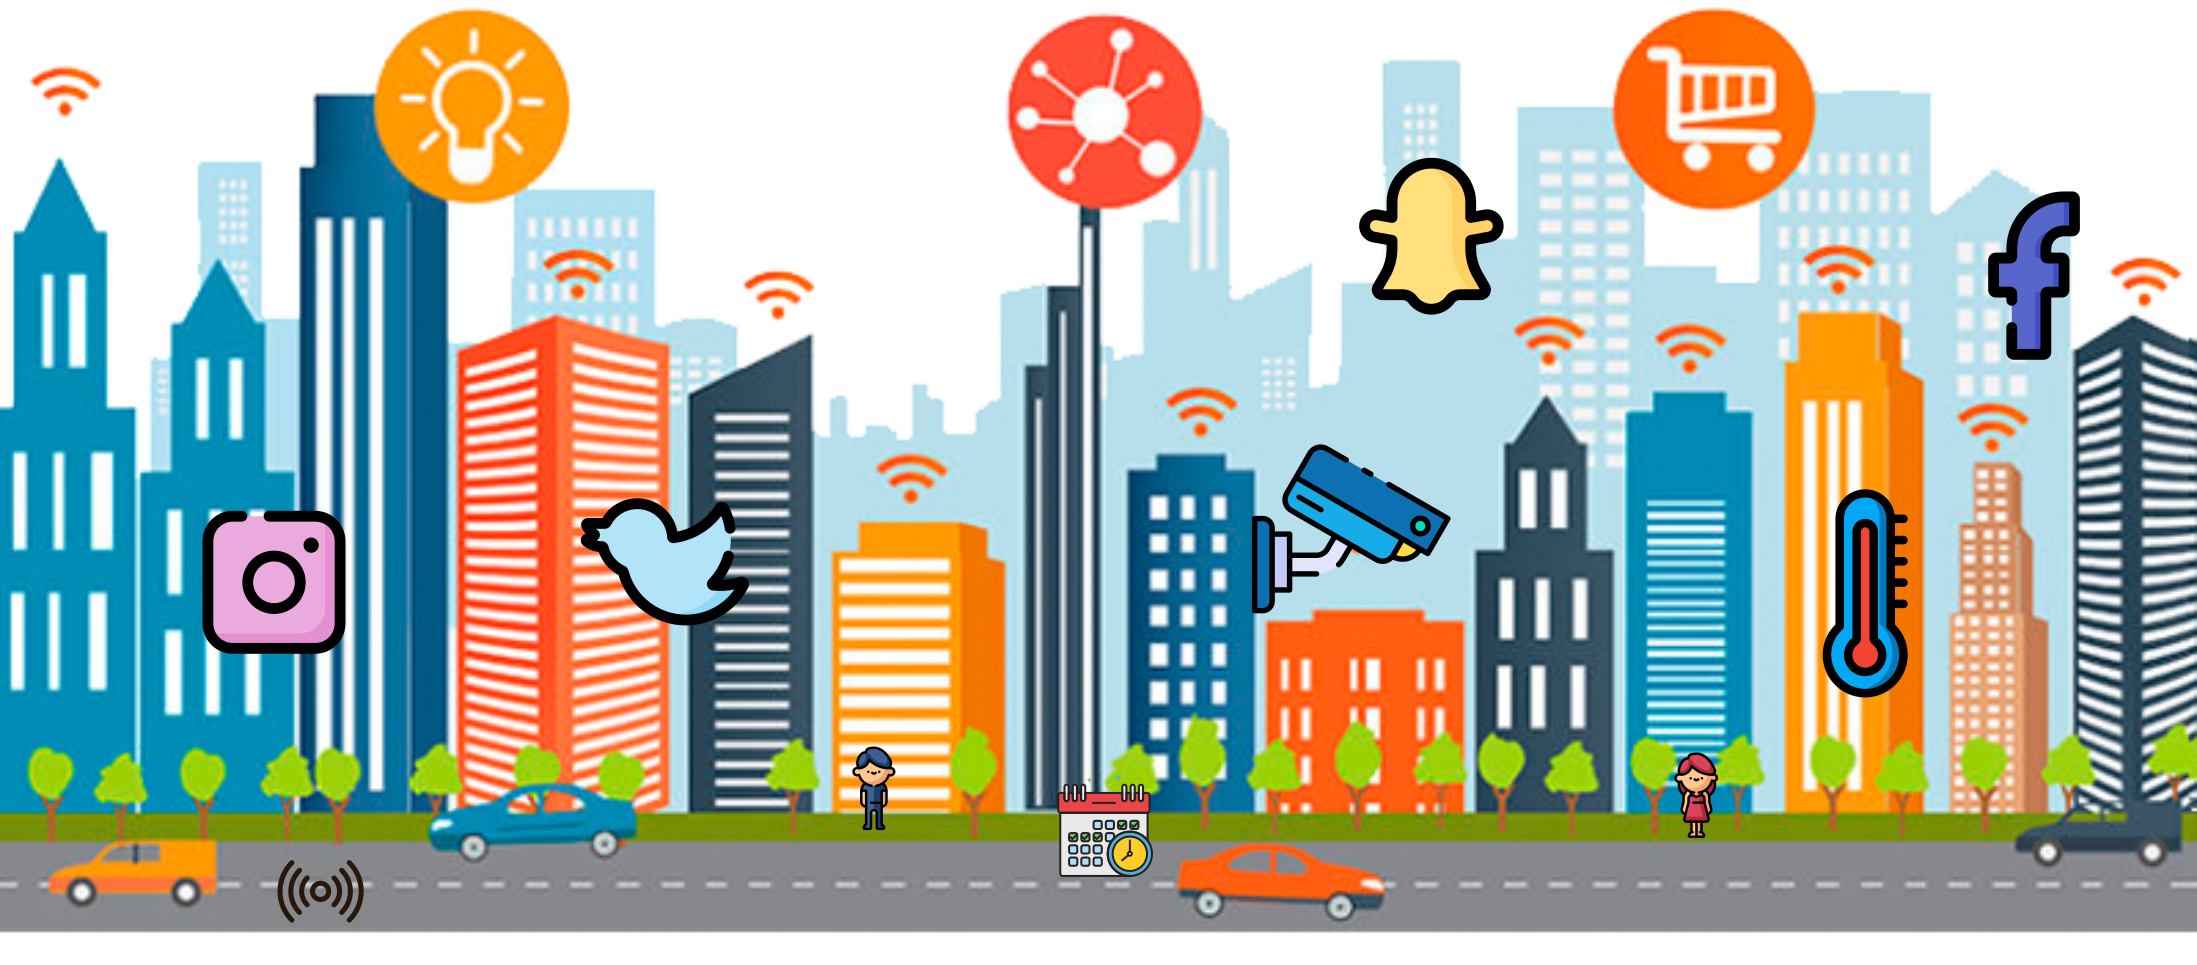
\includegraphics[width=.7\linewidth]{figures/smartcity.png}
\end{figure}
\par A wealth of spatial, social and temporal information in smart cities and smart city simulations
    \begin{itemize}
        \item \textit{How to reduce the number of possible cases?
        \item How to ensure that the agents carry out the actions that are really necessary?}
    \end{itemize}
\alert{$\rightarrow$ An anticipatory reasoning}

\note{
\par Cette richesse d'information se retrouve de manière générale au niveau de la ville intelligente et dons au niveau des simulations multi-agents pour les villes intelligente comme celles sur lesquelles nous travaillons. En effet, une ville intelligente est généralement instrumentée et dispose d'un ensemble de capteurs et d'un ensembles d'outils permettant l'échange d'une grande quantité d'informations spatiales, sociales et temporelles. 
\par Face à cette quantité d'informations phénoménale, nous pensons donc qu'il est indispensable de réduire l'ensemble des cas possibles en dotant les agents d'une capacité d'anticipation. Cela devrait leur permettre d’optimiser leur comportement en n’effectuant ainsi que les actions véritablement nécessaires. 
}
\end{frame}

\begin{frame}{Problem}{Example}

\begin{figure}
    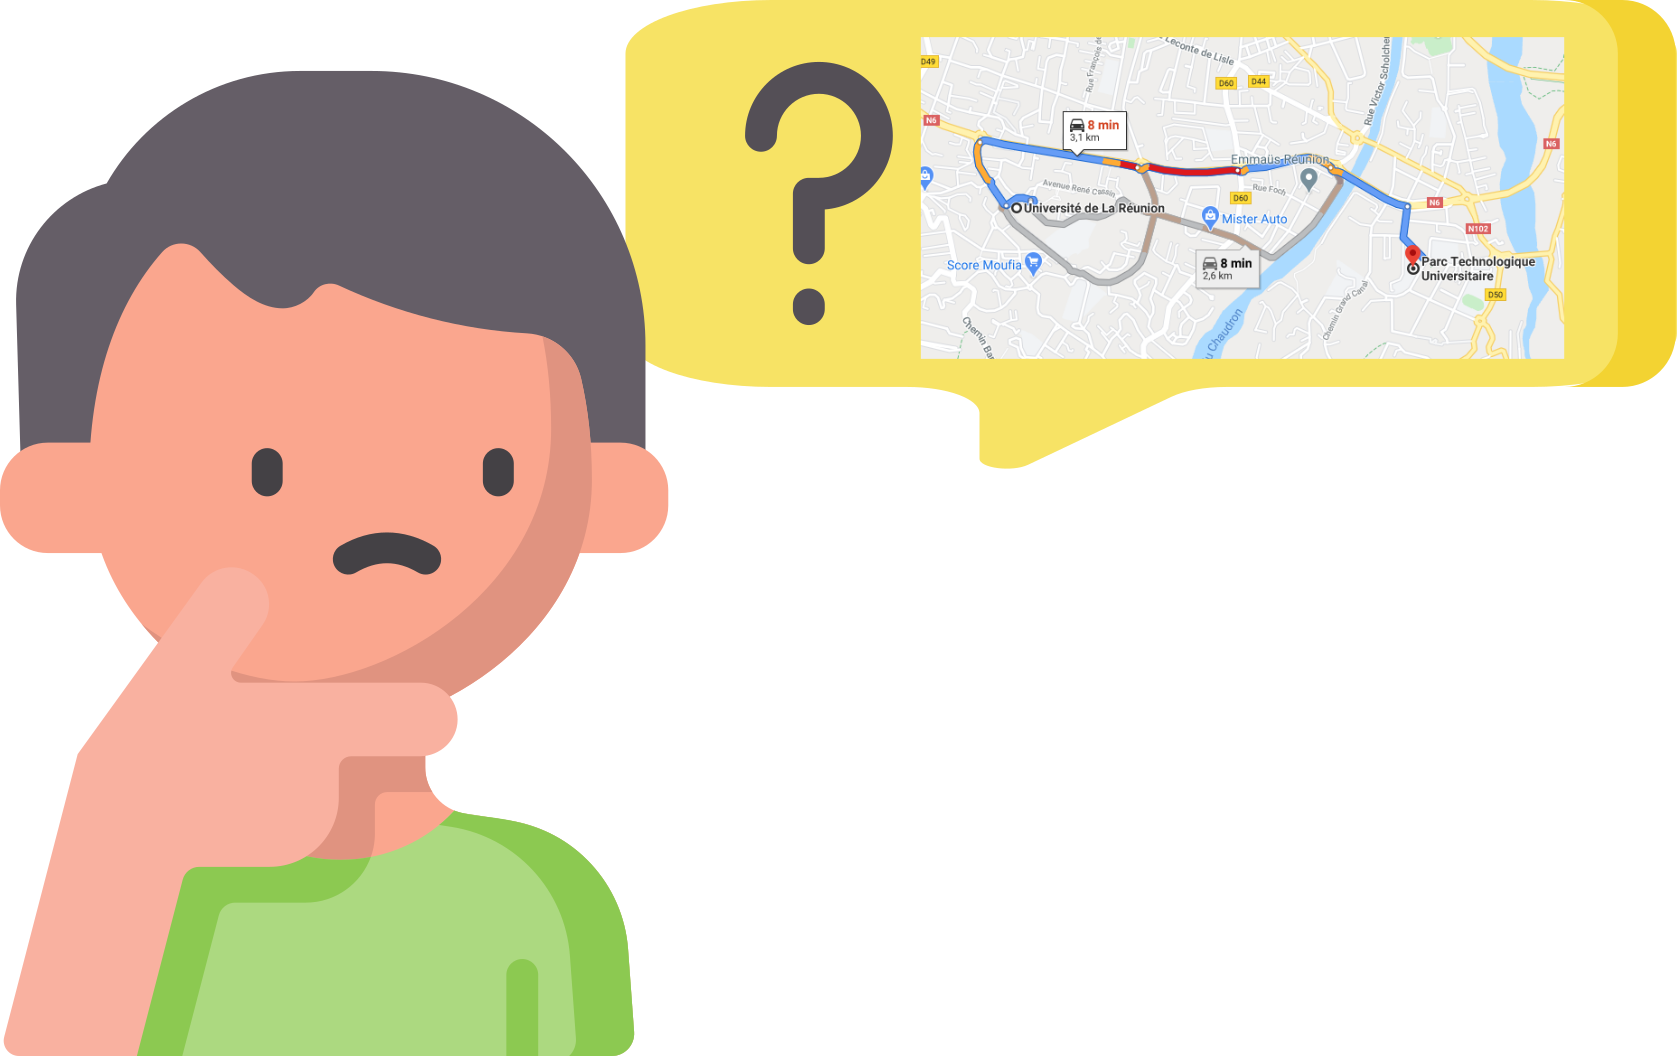
\includegraphics[width=.4\linewidth]{figures/question.png}
    \caption{ Example of the agent's anticipatory reasoning}
\end{figure}
\par The path choice in SmartCityModel or SkuadCityModel is based on the consideration of spatial dimension only: \alert{no consideration of the temporal dimension}
\note{
 Si nous prenons l'exemple du raisonnement anticipatif de l'agent dans SmartCityModel ou dans SkuadCityModel, afin de choisir un chemin parmis une liste de chemin ce dernier utilise une minimisation de la quantité prévisionnelle d'énergie requise pour effectuer le trajet. Pour cela, il prend en compte la valeur de la distance et de la pente. Aucune information temporelles, sur les projets individuelles relatives au planning d'activité des agents n'est pris en compte. Pourtant ce informations existent bel et bien au niveau de la simulation.
}
\end{frame}


\begin{frame}{Problem}{A wealth of untapped information on temporal behaviours}
\begin{enumerate}
    \item A weak consideration of temporal information compared to spatial and social information in multi-agent anticipation reasoning
    \begin{itemize}
        \item \textit{How to use temporal information in the same way as spatial and organisational information?}
    \end{itemize}
\vspace{.5cm}
    \item No consideration of information about the future (project) at the level of anticipatory reasoning
\begin{itemize}
    \item \textit{How can we provide visibility on the future dimension of time?}
\end{itemize}
\vspace{.5cm}
\alert{$\rightarrow$ An environment for the representation of the agents temporal behaviour}
\end{enumerate} 



\note{
\par Ce même constat s'applique de manière plus générale, au niveau de la plupart des raisonnements anticipatifs au niveau des agents dans les SMA. Nous constatons une faible prise en compte de la dimensions temporelle face aux dimensions spatiales et sociales. De plus, si nous nous concentrons particulièrement sur la prise en compte de la dimension temporelle dans le raisonnements anticipatif des agents, dans la majorité des approches que nous pouvons rencontrer dans la littérature, les agents prennent uniquement en compte, dans leur modèle prédictif, les informations sur le passé et sur le présent pour prédire les informations sur le futur. Aucune information sur les projets, sur le planning d'activité (futur) des agents n'est prise en compte. Cela est du au fait qu'il n'existe au sein du système aucune représentation de la dimension temps qui permette aux agents d'avoir une visibilité sur cette dimension futur du temps.
\par Nous pensons alors qu'il est insispensable de mettre en oeuvre, au niveau de la simulation, un support de représentation du comportement temporel relatif au planning d'activité des agents. Ce support devrait permettre l'échange d'information temporel et son exploitation au même titre que les informations spatiales et sociales.
}
\end{frame}

\begin{frame}{Contributions}
\begin{enumerate}
\Huge{
   \centering{ \item A temporal environment}\\}
   \medbreak
     \par \centering{ \normalsize{Temporal representation}\\}
    \par \Huge{\centering{$\Downarrow$}}
    \Huge{
    \centering{\item A consideration of the future information in anticipatory reasonning}\\}
    \centering{\normalsize{Temporal reasoning}}
\end{enumerate}

\note{
\par Face à ces besoins, nous proposons d'améliorer les simulations multi-agents sur deux niveaux:
\begin{itemize}
    \item Au niveau de la représentation du temps : nous proposons de faire évoluer les simulations multi-agents de manière à considérer le temps comme un milieu d'intéraction, au même titre que l'espace et l'organisation. Cela devrait permettre une visibilité sur le comportement temporel des agent, plus particulièrement sur la dynamique d'activation temporelle future des agents.
    \item Au niveau du raisonnement temporel, nous proposons d'enrichir le raisonnement anticipatif des agents par une prise en compte des informations sur la dimension futur du temps permise par la visibilité sur la dimension futur offerte par le support de représentation qui constitue notre première contribution.
\end{itemize}
}
    
\end{frame}